% L13a figure: the request-response cycle of a RESTful web service.
%
% A client sends an HTTPS request (method, URL, headers, body) to the REST API.
% The API routes and validates the request, calls the backend services, and
% sends back an HTTPS response (status code, headers, body). The four numbered
% steps match the four components in the lecture's RESTful Web Services section.
%
% Drawn on November 12, 2026 with the palette and build of the L12c figures.
% It replaces the client / REST API / server screenshot used in the 2025
% lecture's source material. The notebook SVG carries a dark palette added by
% theme_svg.py; keep new colors in that script's mapping when changing the
% palette here.
\documentclass[tikz,border=4pt]{standalone}
\usepackage[no-math]{fontspec}
\IfFontExistsTF{Arial}{\setsansfont{Arial}}{\setsansfont{TeX Gyre Heros}}
\renewcommand{\familydefault}{\sfdefault}
\usepackage{amsmath,amssymb}
\usetikzlibrary{arrows.meta, calc}

% Ink, blue, gray, and band match the L12c figures. Blue marks the request.
\definecolor{vnink}{HTML}{202124}
\definecolor{gdblue}{HTML}{0091FF}
\definecolor{gdgray}{HTML}{6D7278}
\definecolor{waband}{HTML}{EEF0F2}
\definecolor{nodefill}{HTML}{FFFFFF}

\begin{document}
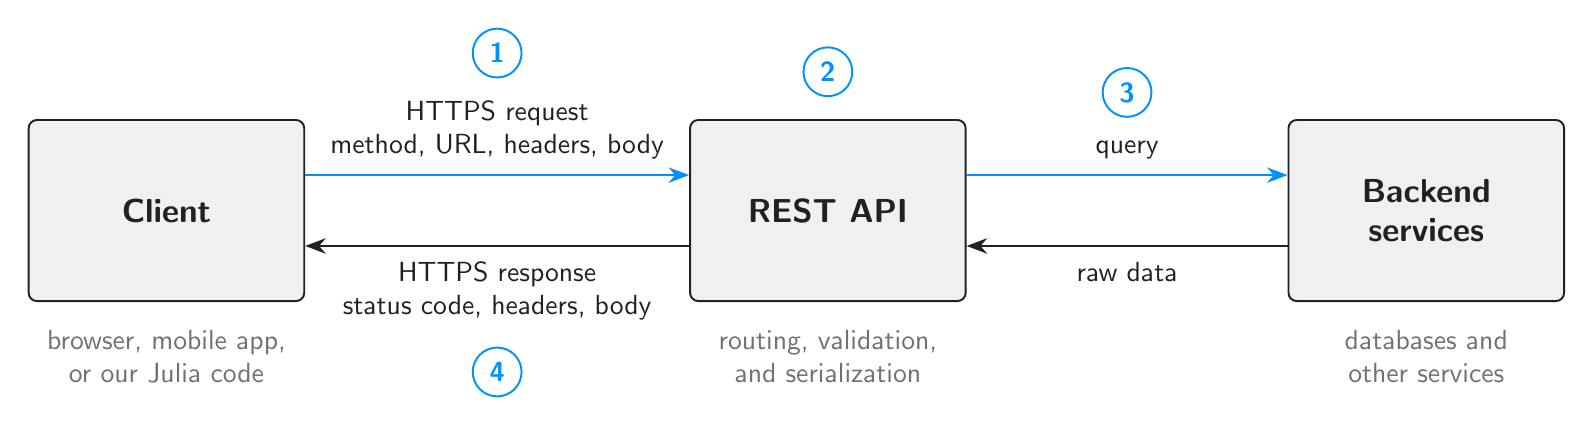
\begin{tikzpicture}[
  font=\sffamily\large,
  >={Stealth[length=2.6mm]},
  box/.style={draw=vnink, rounded corners=3pt, minimum width=3.5cm, minimum height=2.3cm,
    fill=waband, line width=0.7pt, text=vnink, align=center, font=\sffamily\large\bfseries},
  note/.style={font=\sffamily\normalsize, text=gdgray, align=center},
  msg/.style={font=\sffamily\normalsize, text=vnink, align=center},
  stepnum/.style={circle, draw=gdblue, fill=nodefill, line width=0.7pt, inner sep=0pt,
    minimum size=6.2mm, font=\sffamily\normalsize\bfseries, text=gdblue},
  request/.style={->, line width=1.0pt, draw=gdblue},
  response/.style={->, line width=1.0pt, draw=vnink}
]

% ------------------------------------------------------------------ the boxes
\node[box] (client)  at (0.0, 0) {Client};
\node[box] (api)     at (8.4, 0) {REST API};
\node[box] (backend) at (16.0, 0) {Backend\\services};

\node[note] at (0.0, -1.85)  {browser, mobile app,\\or our Julia code};
\node[note] at (8.4, -1.85)  {routing, validation,\\and serialization};
\node[note] at (16.0, -1.85) {databases and\\other services};

% --------------------------------------------------- client <-> API (over HTTPS)
\draw[request]  ($(client.east)+(0, 0.45)$) -- ($(api.west)+(0, 0.45)$)
  node[msg, midway, above=2pt] {HTTPS request\\method, URL, headers, body};
\draw[response] ($(api.west)+(0,-0.45)$) -- ($(client.east)+(0,-0.45)$)
  node[msg, midway, below=2pt] {HTTPS response\\status code, headers, body};

% --------------------------------------------------------- API <-> backend
\draw[request]  ($(api.east)+(0, 0.45)$) -- ($(backend.west)+(0, 0.45)$)
  node[msg, midway, above=2pt] {query};
\draw[response] ($(backend.west)+(0,-0.45)$) -- ($(api.east)+(0,-0.45)$)
  node[msg, midway, below=2pt] {raw data};

% ------------------------------------------------------------ the four steps
\node[stepnum] at ($(client.east)!0.5!(api.west)+(0, 2.00)$) {1};
\node[stepnum] at ($(api.north)+(0, 0.60)$) {2};
\node[stepnum] at ($(api.east)!0.5!(backend.west)+(0, 1.50)$) {3};
\node[stepnum] at ($(client.east)!0.5!(api.west)+(0,-2.05)$) {4};

\end{tikzpicture}
\end{document}
